
\newpage
\null
\thispagestyle{empty}
\newpage
\addcontentsline{toc}{chapter}{Hosea}

% Safely inserts your illustration full-bleed on its own page.
% This completely bypasses the page builder, headers, and geometry bugs!
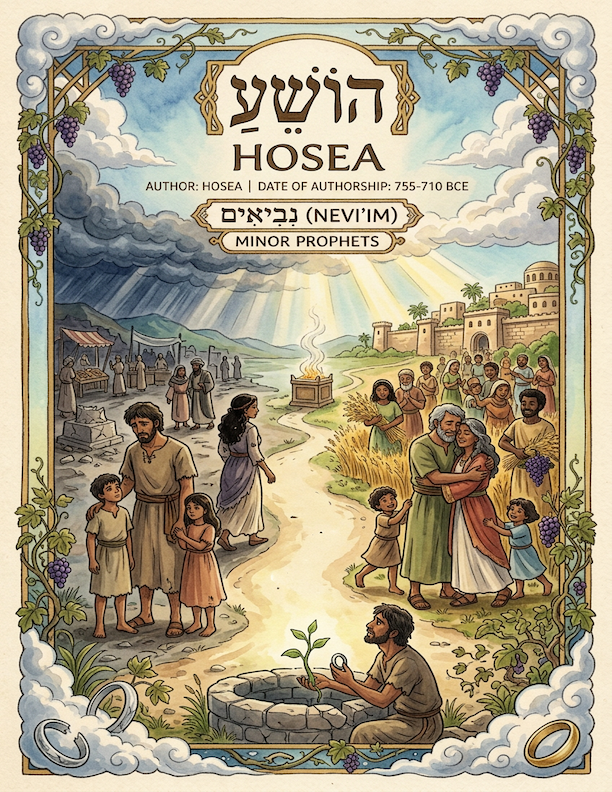
\includepdf[pages=1, fitpaper=false, width=\paperwidth, height=\paperheight, , keepaspectratio=false]{images/divider2/hosea_2.png}
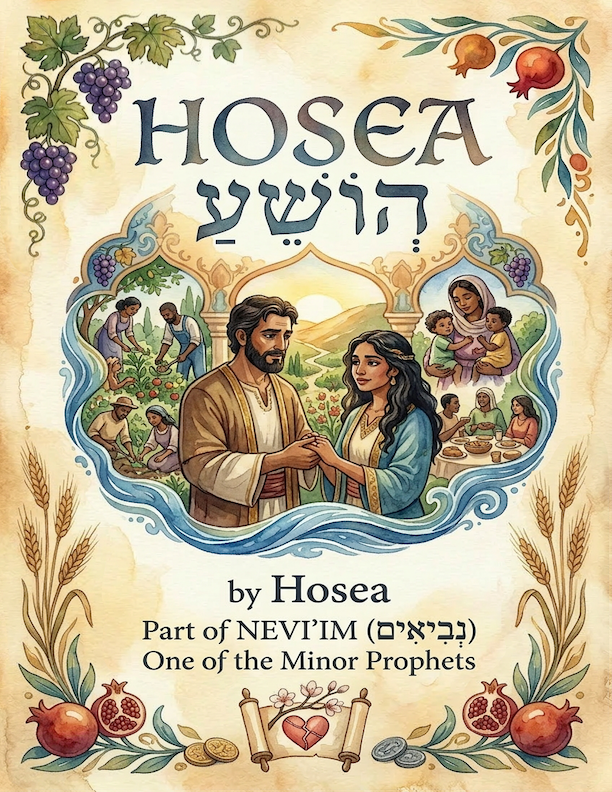
\includepdf[pages=1, fitpaper=false, width=\paperwidth, height=\paperheight, , keepaspectratio=false]{images/divider1/hosea.png}

\includepdf[pages=1, fitpaper=false, width=\paperwidth, height=\paperheight, , keepaspectratio=false]{images/8.5x11-Dot-Grid.png}

\includepdf[pages=1, fitpaper=false, width=\paperwidth, height=\paperheight, , keepaspectratio=false]{images/8.5x11-Dot-Grid.png}

\mybook{Hosea}
\vspace{-1.36in}

% HOSEA 1
\begin{multicols}{2}
\mychapter{} \myverse*{}The LORD’s\footnote{1:1 When rendered in ALL CAPITAL LETTERS, “LORD” or “GOD” is the translation of God’s Proper Name.}
word that came to Hosea the son of Beeri, in the days of Uzziah, Jotham, Ahaz, and Hezekiah, kings of
Judah, and in the days of Jeroboam the son of Joash, king of Israel.

\myverse{}When the LORD spoke at first by Hosea, the LORD said to Hosea,
“Go, take for yourself a wife of prostitution and children of unfaithfulness; for the land commits great
adultery, forsaking the LORD.”

\myverse{}So he went and took Gomer the daughter of Diblaim; and she conceived,
and bore him a son.

\myverse{}The LORD said to him, “Call his name Jezreel, for yet a little
while, and I will avenge the blood of Jezreel on the house of Jehu, and will cause the kingdom of the
house of Israel to cease.
\myverse{}It will happen in that day that I will break the bow of Israel in the valley
of Jezreel.”

\myverse{}She conceived again, and bore a daughter.

Then he said to him, “Call her name Lo-Ruhamah,\footnote{1:6 Lo-Ruhamah means “not loved”.} for I will no longer have mercy on the house of Israel,
that I should in any way pardon them.
\myverse{}But I will have mercy on the house of Judah, and will save them by the LORD
their God,\footnote{1:7 The Hebrew word rendered “God” is “אֱלֹהִ֑ים” (Elohim).} and will not save them
by bow, sword, battle, horses, or horsemen.”

\myverse{}Now when she had weaned Lo-Ruhamah, she conceived, and bore a son.

\myverse{}He said, “Call his name Lo-Ammi,\footnote{1:9 Lo-Ammi means “not my people”.} for you are not my people, and I will not be yours.
\myverse{}Yet the number of the children of Israel will be as the sand of the sea, which
can’t be measured or counted; and it will come to pass that, in the place where it was said to them, ‘You
are not my people,’ they will be called ‘sons of the living God.’
\myverse{}The children of Judah and the children of Israel will be gathered together,
and they will appoint themselves one head, and will go up from the land; for great will be the day of
Jezreel.


% HOSEA 2
\mychapter{} \myverse*{}“Say to your brothers, ‘My people!’\footnote{2:1 ‘Ammi’ in Hebrew}

and to your sisters, ‘My loved one!’\footnote{2:1 ‘Ruhamah’ in Hebrew}

\myverse{}Contend with your mother!

Contend, for she is not my wife,

neither am I her husband;

and let her put away her prostitution from her face,

and her adulteries from between her breasts;

\myverse{}lest I strip her naked,

and make her bare as in the day that she was born,

and make her like a wilderness,

and set her like a dry land,

and kill her with thirst.

\myverse{}Indeed, on her children I will have no mercy,

for they are children of unfaithfulness.

\myverse{}For their mother has played the prostitute.

She who conceived them has done shamefully;

for she said, ‘I will go after my lovers,

who give me my bread and my water,

my wool and my flax,

my oil and my drink.’

\myverse{}Therefore behold,\footnote{2:6 “Behold”, from “הִנֵּה”, means look at, take notice, observe, see, or gaze at. It is
	often used as an interjection.} I will hedge up your way with thorns,

and I will build a wall against her,

that she can’t find her way.

\myverse{}She will follow after her lovers,

but she won’t overtake them;

and she will seek them,

but won’t find them.

Then she will say, ‘I will go and return to my first husband,

for then it was better with me than now.’

\myverse{}For she didn’t know that I gave her the grain, the new wine, and
the oil,

and multiplied to her silver and gold, which they used for Baal.

\myverse{}Therefore I will take back my grain in its time,

and my new wine in its season,

and will pluck away my wool and my flax which should have covered her nakedness.

\myverse{}Now I will uncover her lewdness in the sight of her lovers,

and no one will deliver her out of my hand.

\myverse{}I will also cause all her celebrations to cease:

her feasts, her new moons, her Sabbaths, and all her solemn assemblies.

\myverse{}I will lay waste her vines and her fig trees,

about which she has said, ‘These are my wages that my lovers have given me,’

and I will make them a forest,

and the animals of the field shall eat them.

\myverse{}I will visit on her the days of the Baals,

to which she burned incense

when she decked herself with her earrings and her jewels,

and went after her lovers

and forgot me,” says the LORD.

\myverse{}“Therefore behold, I will allure her,

and bring her into the wilderness,

and speak tenderly to her.

\myverse{}I will give her vineyards from there,

and the valley of Achor for a door of hope;

and she will respond there

as in the days of her youth,

and as in the day when she came up out of the land of Egypt.

\myverse{}It will be in that day,” says the LORD,

“that you will call me ‘my husband,’

and no longer call me ‘my master.’

\myverse{}For I will take away the names of the Baals out of her mouth,

and they will no longer be mentioned by name.

\myverse{}In that day I will make a covenant for them with the animals
of the field,

and with the birds of the sky,

and with the creeping things of the ground.

I will break the bow, the sword, and the battle out of the land,

and will make them lie down safely.

\myverse{}I will betroth you to me forever.

Yes, I will betroth you to me in righteousness, in justice, in loving kindness,
and in compassion.

\myverse{}I will even betroth you to me in faithfulness;

and you shall know the LORD.

\myverse{}It will happen in that day, that I will respond,” says the LORD.

“I will respond to the heavens,

and they will respond to the earth;

\myverse{}and the earth will respond to the grain, and the new
wine, and the oil;

and they will respond to Jezreel.

\myverse{}I will sow her to me in the earth;

and I will have mercy on her who had not obtained mercy;

and I will tell those who were not my people, ‘You are my people;’

and they will say, ‘You are My God!’ ”


%HOSEA 3
\mychapter{} \myverse*{}The LORD said to me, “Go again, love a woman loved by another,
and an adulteress, even as the LORD loves the children of Israel, though they turn to other gods, and
love cakes of raisins.”

\myverse{}So I bought her for myself for fifteen pieces of silver and a homer\footnote{3:2 1 homer is about 220 liters or 6 bushels} and a half of barley.
\myverse{}I said to her, “You shall stay with me many days. You shall not play the prostitute,
and you shall not be with any other man. I will also be so toward you.”

\myverse{}For the children of Israel shall live many days without king, without
prince, without sacrifice, without sacred stone, and without ephod or idols.
\myverse{}Afterward the children of Israel shall return and seek the LORD their God, and
David their king, and shall come with trembling to the LORD and to his blessings in the last days.


% HOSEA 4 
\mychapter{} \myverse*{}Hear the LORD’s word, you children of Israel,

for the LORD has a charge against the inhabitants of the land:

“Indeed there is no truth, nor goodness,

nor knowledge of God in the land.

\myverse{}There is cursing, lying, murder, stealing, and committing adultery;

they break boundaries, and bloodshed causes bloodshed.

\myverse{}Therefore the land will mourn,

and everyone who dwells in it will waste away,

with all living things in her,

even the animals of the field and the birds of the sky;

yes, the fish of the sea also die.


\vspace{\baselineskip} \myverse{}“Yet let no man bring a charge, neither let any man accuse;

for your people are like those who bring charges against a priest.

\myverse{}You will stumble in the day,

and the prophet will also stumble with you in the night;

and I will destroy your mother.

\myverse{}My people are destroyed for lack of knowledge.

Because you have rejected knowledge, I will also reject you,

that you may be no priest to me.

Because you have forgotten your God’s Torah,

I will also forget your children.

\myverse{}As they were multiplied, so they sinned against me.

I will change their glory into shame.

\myverse{}They feed on the sin of my people,

and set their heart on their iniquity.

\myverse{}It will be like people, like priest;

and I will punish them for their ways,

and will repay them for their deeds.

\myverse{}They will eat, and not have enough.

They will play the prostitute, and will not increase;

because they have abandoned listening to the LORD.

\myverse{}Prostitution, wine, and new wine take away understanding.

\myverse{}My people consult with their wooden idol,

and answer to a stick of wood.

Indeed the spirit of prostitution has led them astray,

and they have been unfaithful to their God.

\myverse{}They sacrifice on the tops of the mountains,

and burn incense on the hills, under oaks, poplars, and terebinths,

because its shade is good.

Therefore your daughters play the prostitute,

and your brides commit adultery.

\myverse{}I will not punish your daughters when they play the prostitute,

nor your brides when they commit adultery;

because the men consort with prostitutes,

and they sacrifice with the shrine prostitutes;

so the people without understanding will come to ruin.


\vspace{\baselineskip} \myverse{}“Though you, Israel, play the prostitute,

yet don’t let Judah offend;

and don’t come to Gilgal,

neither go up to Beth Aven,

nor swear, ‘As the LORD lives.’

\myverse{}For Israel has behaved extremely stubbornly, like a stubborn
heifer.

Then how will the LORD feed them like a lamb in a meadow?

\myverse{}Ephraim is joined to idols.

Leave him alone!

\myverse{}Their drink has become sour.

They play the prostitute continually.

Her rulers dearly love their shameful way.

\myverse{}The wind has wrapped her up in its wings;

and they shall be disappointed because of their sacrifices.


% HOSEA 5
\mychapter{} \myverse*{}“Listen to this, you priests!

Listen, house of Israel,

and give ear, house of the king!

For the judgment is against you;

for you have been a snare at Mizpah,

and a net spread on Tabor.

\myverse{}The rebels are deep in slaughter,

but I discipline all of them.

\myverse{}I know Ephraim,

and Israel is not hidden from me;

for now, Ephraim, you have played the prostitute.

Israel is defiled.

\myverse{}Their deeds won’t allow them to turn to their God,

for the spirit of prostitution is within them,

and they don’t know the LORD.

\myverse{}The pride of Israel testifies to his face.

Therefore Israel and Ephraim will stumble in their iniquity.

Judah also will stumble with them.

\myverse{}They will go with their flocks and with their herds to seek the
LORD,

but they won’t find him.

He has withdrawn himself from them.

\myverse{}They are unfaithful to the LORD;

for they have borne illegitimate children.

Now the new moon will devour them with their fields.


\vspace{\baselineskip} \myverse{}“Blow the cornet in Gibeah,

and the shofar in Ramah!

Sound a battle cry at Beth Aven, behind you, Benjamin!

\myverse{}Ephraim will become a desolation in the day of rebuke.

Among the tribes of Israel, I have made known that which will surely be.

\myverse{}The princes of Judah are like those who remove a landmark.

I will pour out my wrath on them like water.

\myverse{}Ephraim is oppressed,

he is crushed in judgment,

because he is intent in his pursuit of idols.

\myverse{}Therefore I am to Ephraim like a moth,

and to the house of Judah like rottenness.


\vspace{\baselineskip} \myverse{}“When Ephraim saw his sickness,

and Judah his wound,

then Ephraim went to Assyria,

and sent to King Jareb:

but he is not able to heal you,

neither will he cure you of your wound.

\myverse{}For I will be to Ephraim like a lion,

and like a young lion to the house of Judah.

I myself will tear in pieces and go away.

I will carry off, and there will be no one to deliver.

\myverse{}I will go and return to my place,

until they acknowledge their offense,

and seek my face.

In their affliction they will seek me earnestly.”


%Hosea 6
\mychapter{} \myverse*{}“Come! Let’s return to the LORD;

for he has torn us to pieces,

and he will heal us;

he has injured us,

and he will bind up our wounds.

\myverse{}After two days he will revive us.

On the third day he will raise us up,

and we will live before him.

\myverse{}Let’s acknowledge the LORD.

Let’s press on to know the LORD.

As surely as the sun rises,

the LORD will appear.

He will come to us like the rain,

like the spring rain that waters the earth.”


\vspace{\baselineskip} \myverse{}“Ephraim, what shall I do to you?

Judah, what shall I do to you?

For your love is like a morning cloud,

and like the dew that disappears early.

\myverse{}Therefore I have cut them to pieces with the prophets;

I killed them with the words of my mouth.

Your judgments are like a flash of lightning.

\myverse{}For I desire mercy, and not sacrifice;

and the knowledge of God more than burnt offerings.

\myverse{}But they, like Adam, have broken the covenant.

They were unfaithful to me there.

\myverse{}Gilead is a city of those who work iniquity;

it is stained with blood.

\myverse{}As gangs of robbers wait to ambush a man,

so the company of priests murder on the path toward Shechem,

committing shameful crimes.

\myverse{}In the house of Israel I have seen a horrible thing.

There is prostitution in Ephraim.

Israel is defiled.


\vspace{\baselineskip} \myverse{}“Also, Judah, there is a harvest appointed for you,

when I restore the fortunes of my people.


%HOSEA 7
\mychapter{} \myverse*{}When I would heal Israel,

then the iniquity of Ephraim is uncovered,

also the wickedness of Samaria;

for they commit falsehood,

and the thief enters in,

and the gang of robbers ravages outside.

\myverse{}They don’t consider in their hearts that I remember all their
wickedness.

Now their own deeds have engulfed them.

They are before my face.

\myverse{}They make the king glad with their wickedness,

and the princes with their lies.

\myverse{}They are all adulterers.

They are burning like an oven that the baker stops stirring,

from the kneading of the dough, until it is leavened.

\myverse{}On the day of our king, the princes made themselves sick with
the heat of wine.

He joined his hand with mockers.

\myverse{}For they have prepared their heart like an oven,

while they lie in wait.

Their anger smolders all night.

In the morning it burns as a flaming fire.

\myverse{}They are all hot as an oven,

and devour their judges.

All their kings have fallen.

There is no one among them who calls to me.

\myverse{}Ephraim mixes himself among the nations.

Ephraim is a pancake not turned over.

\myverse{}Strangers have devoured his strength,

and he doesn’t realize it.

Indeed, gray hairs are here and there on him,

and he doesn’t realize it.

\myverse{}The pride of Israel testifies to his face;

yet they haven’t returned to the LORD their God,

nor sought him, for all this.


\vspace{\baselineskip} \myverse{}“Ephraim is like an easily deceived dove, without understanding.

They call to Egypt.

They go to Assyria.

\myverse{}When they go, I will spread my net on them.

I will bring them down like the birds of the sky.

I will chastise them, as their congregation has heard.

\myverse{}Woe to them!

For they have wandered from me.

Destruction to them!

For they have trespassed against me.

Though I would redeem them,

yet they have spoken lies against me.

\myverse{}They haven’t cried to me with their heart,

but they howl on their beds.

They assemble themselves for grain and new wine.

They turn away from me.

\myverse{}Though I have taught and strengthened their arms,

yet they plot evil against me.

\myverse{}They return, but not to the Most High.

They are like a faulty bow.

Their princes will fall by the sword for the rage of their tongue.

This will be their derision in the land of Egypt.


% HOSEA 8
\mychapter{} \myverse*{}“Put the shofar to your lips!

Something like an eagle is over the LORD’s house,

because they have broken my covenant

and rebelled against my law.

\myverse{}They cry to me, ‘My God, we, Israel, acknowledge you!’

\myverse{}Israel has cast off that which is good.

The enemy will pursue him.

\myverse{}They have set up kings, but not by me.

They have made princes, and I didn’t approve.

Of their silver and their gold they have made themselves idols,

that they may be cut off.

\myverse{}Let Samaria throw out his calf idol!

My anger burns against them!

How long will it be until they are capable of purity?

\myverse{}For this is even from Israel!

The workman made it, and it is no God;

indeed, the calf of Samaria shall be broken in pieces.

\myverse{}For they sow the wind,

and they will reap the whirlwind.

He has no standing grain.

The stalk will yield no head.

If it does yield, strangers will swallow it up.

\myverse{}Israel is swallowed up.

Now they are among the nations like a worthless thing.

\myverse{}For they have gone up to Assyria,

like a wild donkey wandering alone.

Ephraim has hired lovers for himself.

\myverse{}But although they sold themselves among the nations,

I will now gather them;

and they begin to waste away because of the oppression of the king of mighty ones.

\myverse{}Because Ephraim has multiplied altars for sinning,

they became for him altars for sinning.

\myverse{}I wrote for him the many things of my law,

but they were regarded as a strange thing.

\myverse{}As for the sacrifices of my offerings,

they sacrifice meat and eat it,

but the LORD doesn’t accept them.

Now he will remember their iniquity,

and punish their sins.

They will return to Egypt.

\myverse{}For Israel has forgotten his Maker and built palaces;

and Judah has multiplied fortified cities;

but I will send a fire on his cities,

and it will devour its fortresses.”


%HOSEA 9
\mychapter{} \myverse*{}Don’t rejoice, Israel, to jubilation like the nations;

for you were unfaithful to your God.

You love the wages of a prostitute at every grain threshing floor.

\myverse{}The threshing floor and the wine press won’t feed them,

and the new wine will fail her.

\myverse{}They won’t dwell in the LORD’s land;

but Ephraim will return to Egypt,

and they will eat unclean food in Assyria.

\myverse{}They won’t pour out wine offerings to the LORD,

neither will they be pleasing to him.

Their sacrifices will be to them like the bread of mourners;

all who eat of it will be polluted;

for their bread will be for their appetite.

It will not come into the LORD’s house.

\myverse{}What will you do in the day of solemn assembly,

and in the day of the feast of the LORD?

\myverse{}For, behold, when they flee destruction,

Egypt will gather them up.

Memphis will bury them.

Nettles will possess their pleasant things of silver.

Thorns will be in their tents.

\myverse{}The days of visitation have come.

The days of reckoning have come.

Israel will consider the prophet to be a fool,

and the man who is inspired to be insane,

because of the abundance of your sins,

and because your hostility is great.

\myverse{}A prophet watches over Ephraim with my God.

A fowler’s snare is on all of his paths,

and hostility in the house of his God.

\myverse{}They have deeply corrupted themselves,

as in the days of Gibeah.

He will remember their iniquity.

He will punish them for their sins.

\myverse{}I found Israel like grapes in the wilderness.

I saw your fathers as the first ripe in the fig tree at its first season;

but they came to Baal Peor, and consecrated themselves to the shameful thing,

and became abominable like that which they loved.

\myverse{}As for Ephraim, their glory will fly away like a bird.

There will be no birth, no one with child, and no conception.

\myverse{}Though they bring up their children,

yet I will bereave them, so that not a man shall be left.

Indeed, woe also to them when I depart from them!

\myverse{}I have seen Ephraim, like Tyre, planted in a pleasant place;

but Ephraim will bring out his children to the murderer.

\myverse{}Give them—LORD what will you give?

Give them a miscarrying womb and dry breasts.


\vspace{\baselineskip} \myverse{}“All their wickedness is in Gilgal;

for there I hated them.

Because of the wickedness of their deeds, I will drive them out of my house!

I will love them no more.

All their princes are rebels.

\myverse{}Ephraim is struck.

Their root has dried up.

They will bear no fruit.

Even though they give birth, yet I will kill the beloved ones of their womb.”


\vspace{\baselineskip} \myverse{}My God will cast them away, because they didn’t listen to him;

and they will be wanderers among the nations.


% HOSEA 10
\mychapter{} \myverse*{}Israel is a luxuriant vine that produces his fruit.

\quad\quad According to the abundance of his fruit he has multiplied his altars.

As their land has prospered, they have adorned their sacred stones.

\myverse{}Their heart is divided.

Now they will be found guilty.

He will demolish their altars.

He will destroy their sacred stones.

\myverse{}Surely now they will say, “We have no king; for we don’t fear
the LORD;

and the king, what can he do for us?”

\myverse{}They make promises, swearing falsely in making covenants.

Therefore judgment springs up like poisonous weeds in the furrows of the field.

\myverse{}The inhabitants of Samaria will be in terror for the calves of
Beth Aven,

for its people will mourn over it,

along with its priests who rejoiced over it,

for its glory, because it has departed from it.

\myverse{}It also will be carried to Assyria for a present to a great king.

Ephraim will receive shame,

and Israel will be ashamed of his own counsel.

\myverse{}Samaria and her king float away

like a twig on the water.

\myverse{}The high places also of Aven, the sin of Israel, will be destroyed.

The thorn and the thistle will come up on their altars.

They will tell the mountains, “Cover us!” and the hills, “Fall on us!”


\vspace{\baselineskip} \myverse{}“Israel, you have sinned from the days of Gibeah.

There they remained.

The battle against the children of iniquity doesn’t overtake them in Gibeah.

\myverse{}When it is my desire, I will chastise them;

and the nations will be gathered against them

when they are bound to their two transgressions.

\myverse{}Ephraim is a trained heifer that loves to thresh,

so I will put a yoke on her beautiful neck.

I will set a rider on Ephraim.

Judah will plow.

Jacob will break his clods.

\myverse{}Sow to yourselves in righteousness,

reap according to kindness.

Break up your fallow ground,

for it is time to seek the LORD,

until he comes and rains righteousness on you.

\myverse{}You have plowed wickedness.

You have reaped iniquity.

You have eaten the fruit of lies,

for you trusted in your way, in the multitude of your mighty men.

\myverse{}Therefore a battle roar will arise among your people,

and all your fortresses will be destroyed,

as Shalman destroyed Beth Arbel in the day of battle.

The mother was dashed in pieces with her children.

\myverse{}So Bethel will do to you because of your great wickedness.

At daybreak the king of Israel will be destroyed.


% HOSEA 11
\mychapter{} \myverse*{}“When Israel was a child, then I loved him,

\quad\quad and called my son out of Egypt.

\myverse{}They called to them, so they went from them.

They sacrificed to the Baals,

and burned incense to engraved images.

\myverse{}Yet I taught Ephraim to walk.

I took them by their arms,

but they didn’t know that I healed them.

\myverse{}I drew them with cords of a man, with ties of love;

and I was to them like those who lift up the yoke on their necks;

and I bent down to him and I fed him.


\vspace{\baselineskip} \myverse{}“They won’t return into the land of Egypt;

but the Assyrian will be their king,

because they refused to repent.

\myverse{}The sword will fall on their cities,

and will destroy the bars of their gates,

and will put an end to their plans.

\myverse{}My people are determined to turn from me.

Though they call to the Most High,

he certainly won’t exalt them.


\vspace{\baselineskip} \myverse{}“How can I give you up, Ephraim?

How can I hand you over, Israel?

How can I make you like Admah?

How can I make you like Zeboiim?

My heart is turned within me,

my compassion is aroused.

\myverse{}I will not execute the fierceness of my anger.

I will not return to destroy Ephraim,

for I am God, and not man—the Holy One among you.

I will not come in wrath.

\myverse{}They will walk after the LORD,

who will roar like a lion;

for he will roar, and the children will come trembling from the west.

\myverse{}They will come trembling like a bird out of Egypt,

and like a dove out of the land of Assyria;

and I will settle them in their houses,” says the LORD.


\vspace{\baselineskip} \myverse{}Ephraim surrounds me with falsehood,

and the house of Israel with deceit.

Judah still strays from God,

and is unfaithful to the Holy One.


% HOSEA 12
\mychapter{} \myverse*{}Ephraim feeds on wind,

\quad\quad and chases the east wind.

He continually multiplies lies and desolation.

They make a covenant with Assyria,

and oil is carried into Egypt.

\myverse{}The LORD also has a controversy with Judah,

and will punish Jacob according to his ways;

according to his deeds he will repay him.

\myverse{}In the womb he took his brother by the heel,

and in his manhood he contended with God.

\myverse{}Indeed, he struggled with the angel, and prevailed;

he wept, and made supplication to him.

He found him at Bethel, and there he spoke with us—

\myverse{}even the LORD, the God of Hosts.

The LORD is his name of renown!

\myverse{}Therefore turn to your God.

Keep kindness and justice,

and wait continually for your God.


\vspace{\baselineskip} \myverse{}A merchant has dishonest scales in his hand.

He loves to defraud.

\myverse{}Ephraim said, “Surely I have become rich.

I have found myself wealth.

In all my wealth they won’t find in me any iniquity that is sin.”


\vspace{\baselineskip} \myverse{}“But I am the LORD your God from the land of Egypt.

I will yet again make you dwell in tents,

as in the days of the solemn feast.

\myverse{}I have also spoken to the prophets,

and I have multiplied visions;

and by the ministry of the prophets I have used parables.

\myverse{}If Gilead is wicked,

surely they are worthless.

In Gilgal they sacrifice bulls.

Indeed, their altars are like heaps in the furrows of the field.

\myverse{}Jacob fled into the country of Aram.

Israel served to get a wife.

For a wife he tended flocks and herds.

\myverse{}By a prophet the LORD brought Israel up out of Egypt,

and by a prophet he was preserved.

\myverse{}Ephraim has bitterly provoked anger.

Therefore his blood will be left on him,

and his Lord\footnote{12:14 The word translated “Lord” (mixed case) is “Adonai.”} will repay his contempt.


%HOSEA 13
\mychapter{} \myverse*{}When Ephraim spoke, there was trembling.

\quad\quad He exalted himself in Israel,

but when he became guilty through Baal, he died.

\myverse{}Now they sin more and more,

and have made themselves molten images of their silver,

even idols according to their own understanding,

all of them the work of the craftsmen.

They say of them, ‘They offer human sacrifice and kiss the calves.’

\myverse{}Therefore they will be like the morning mist,

like the dew that passes away early,

like the chaff that is driven with the whirlwind out of the threshing floor,

and like the smoke out of the chimney.


\vspace{\baselineskip} \myverse{}“Yet I am the LORD your God from the land of Egypt;

and you shall acknowledge no god but me,

and besides me there is no savior.

\myverse{}I knew you in the wilderness,

in the land of great drought.

\myverse{}According to their pasture, so were they filled;

they were filled, and their heart was exalted.

Therefore they have forgotten me.

\myverse{}Therefore I am like a lion to them.

Like a leopard, I will lurk by the path.

\myverse{}I will meet them like a bear that is bereaved of her cubs,

and will tear the covering of their heart.

There I will devour them like a lioness.

The wild animal will tear them.

\myverse{}You are destroyed, Israel, because you are against me,

against your helper.

\myverse{}Where is your king now, that he may save you in all your cities?

And your judges, of whom you said, ‘Give me a king and princes’?

\myverse{}I have given you a king in my anger,

and have taken him away in my wrath.

\myverse{}The guilt of Ephraim is stored up.

His sin is stored up.

\myverse{}The sorrows of a travailing woman will come on him.

He is an unwise son,

for when it is time, he doesn’t come to the opening of the womb.

\myverse{}I will ransom them from the power of Sheol.\footnote{13:14 Sheol is the place of the dead.}

I will redeem them from death!

Death, where are your plagues?

Sheol, where is your destruction?

\vspace{\baselineskip} 
“Compassion will be hidden from my eyes.

\myverse{}Though he is fruitful among his brothers, an east
wind will come,

the breath of the LORD coming up from the wilderness;

and his spring will become dry,

and his fountain will be dried up.

He will plunder the storehouse of treasure.

\myverse{}Samaria will bear her guilt,

for she has rebelled against her God.

They will fall by the sword.

Their infants will be dashed in pieces,

and their pregnant women will be ripped open.”

%HOSEA 14
\mychapter{} \myverse*{}Israel, return to the LORD your God;

\quad\quad for you have fallen because of your sin.

\myverse{}Take words with you, and return to the LORD.

Tell him, “Forgive all our sins,

and accept that which is good;

so we offer bulls as we vowed of our lips.

\myverse{}Assyria can’t save us.

We won’t ride on horses;

neither will we say any more to the work of our hands, ‘Our gods!’

for in you the fatherless finds mercy.”


\vspace{\baselineskip} \myverse{}“I will heal their waywardness.

I will love them freely;

for my anger is turned away from them.

\myverse{}I will be like the dew to Israel.

He will blossom like the lily,

and send down his roots like Lebanon.

\myverse{}His branches will spread,

and his beauty will be like the olive tree,

and his fragrance like Lebanon.

\myverse{}Men will dwell in his shade.

They will revive like the grain,

and blossom like the vine.

Their fragrance will be like the wine of Lebanon.

\myverse{}Ephraim, what have I to do any more with idols?

I answer, and will take care of him.

I am like a green cypress tree;

from me your fruit is found.”


\vspace{\baselineskip} \myverse{}Who is wise, that he may understand these things?

Who is prudent, that he may know them?

For the ways of the LORD are right,

and the righteous walk in them,

but the rebellious stumble in them.

\end{multicols}
